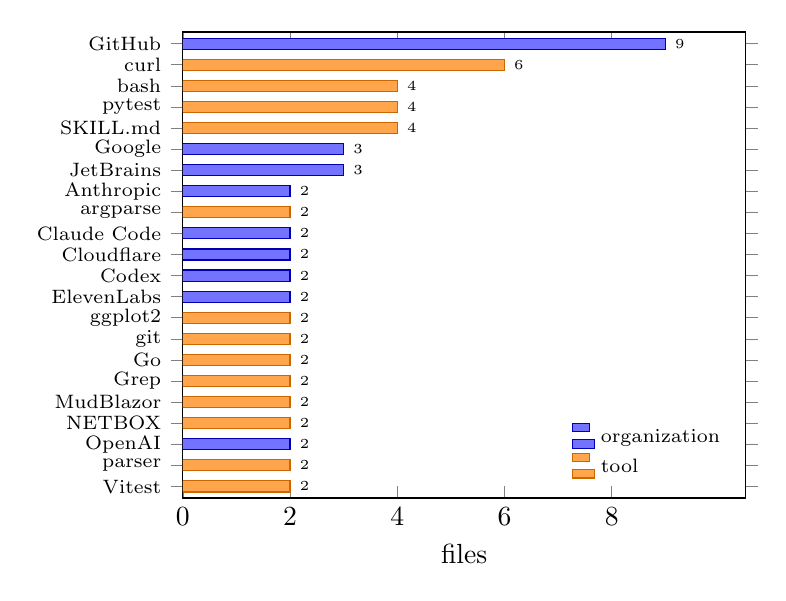
\begin{tikzpicture}
\begin{axis}[
  xbar,
  width=0.72\textwidth,
  height=7.5cm,
  bar width=4pt,
  bar shift=0pt,
  enlarge y limits={abs=0.55},
  xmin=0,
  xmax=10.5,
  xtick={0,2,4,6,8},
  xlabel={files},
  ylabel={},
  ytick={1,...,22},
  yticklabels={
    Vitest,
    parser,
    OpenAI,
    NETBOX,
    MudBlazor,
    Grep,
    Go,
    git,
    ggplot2,
    ElevenLabs,
    Codex,
    Cloudflare,
    Claude Code,
    argparse,
    Anthropic,
    JetBrains,
    Google,
    SKILL.md,
    pytest,
    bash,
    curl,
    GitHub
  },
  yticklabel style={font=\scriptsize, anchor=east},
  nodes near coords,
  every node near coord/.append style={font=\tiny},
  nodes near coords align={horizontal},
  legend style={
    at={(0.98,0.02)},
    anchor=south east,
    font=\scriptsize,
    cells={anchor=west},
    draw=none,
    fill=none
  },
  legend cell align=left,
]
% y=22 is GitHub at the top of the chart.
\addplot[fill=blue!55, draw=blue!70!black] coordinates {
  (9,22)
  (3,17)
  (3,16)
  (2,15)
  (2,13)
  (2,12)
  (2,11)
  (2,10)
  (2,3)
};
\addplot[fill=orange!70, draw=orange!80!black] coordinates {
  (6,21)
  (4,20)
  (4,19)
  (4,18)
  (2,14)
  (2,9)
  (2,8)
  (2,7)
  (2,6)
  (2,5)
  (2,4)
  (2,2)
  (2,1)
};
\legend{organization,tool}
\end{axis}
\end{tikzpicture}
